\section{Results and Discussion}
\label{sec:results}
This section presents evaluation results for the Abilene, GÉANT, and Germany50 topologies using real measured operator traffic. The results emphasize two performance indicators and the reward trade-offs the trained policy makes on networks it has not seen. For the reinforcement learning method, results are reported as mean $\pm$ standard deviation \emph{across model seeds}, each seed contributing its own mean over the retained matrices. Figure~\ref{fig:heatmap} summarises all three metrics for the four methods across both regimes; the sections that follow examine each metric in turn.

\begin{figure}[t]
  \centering
  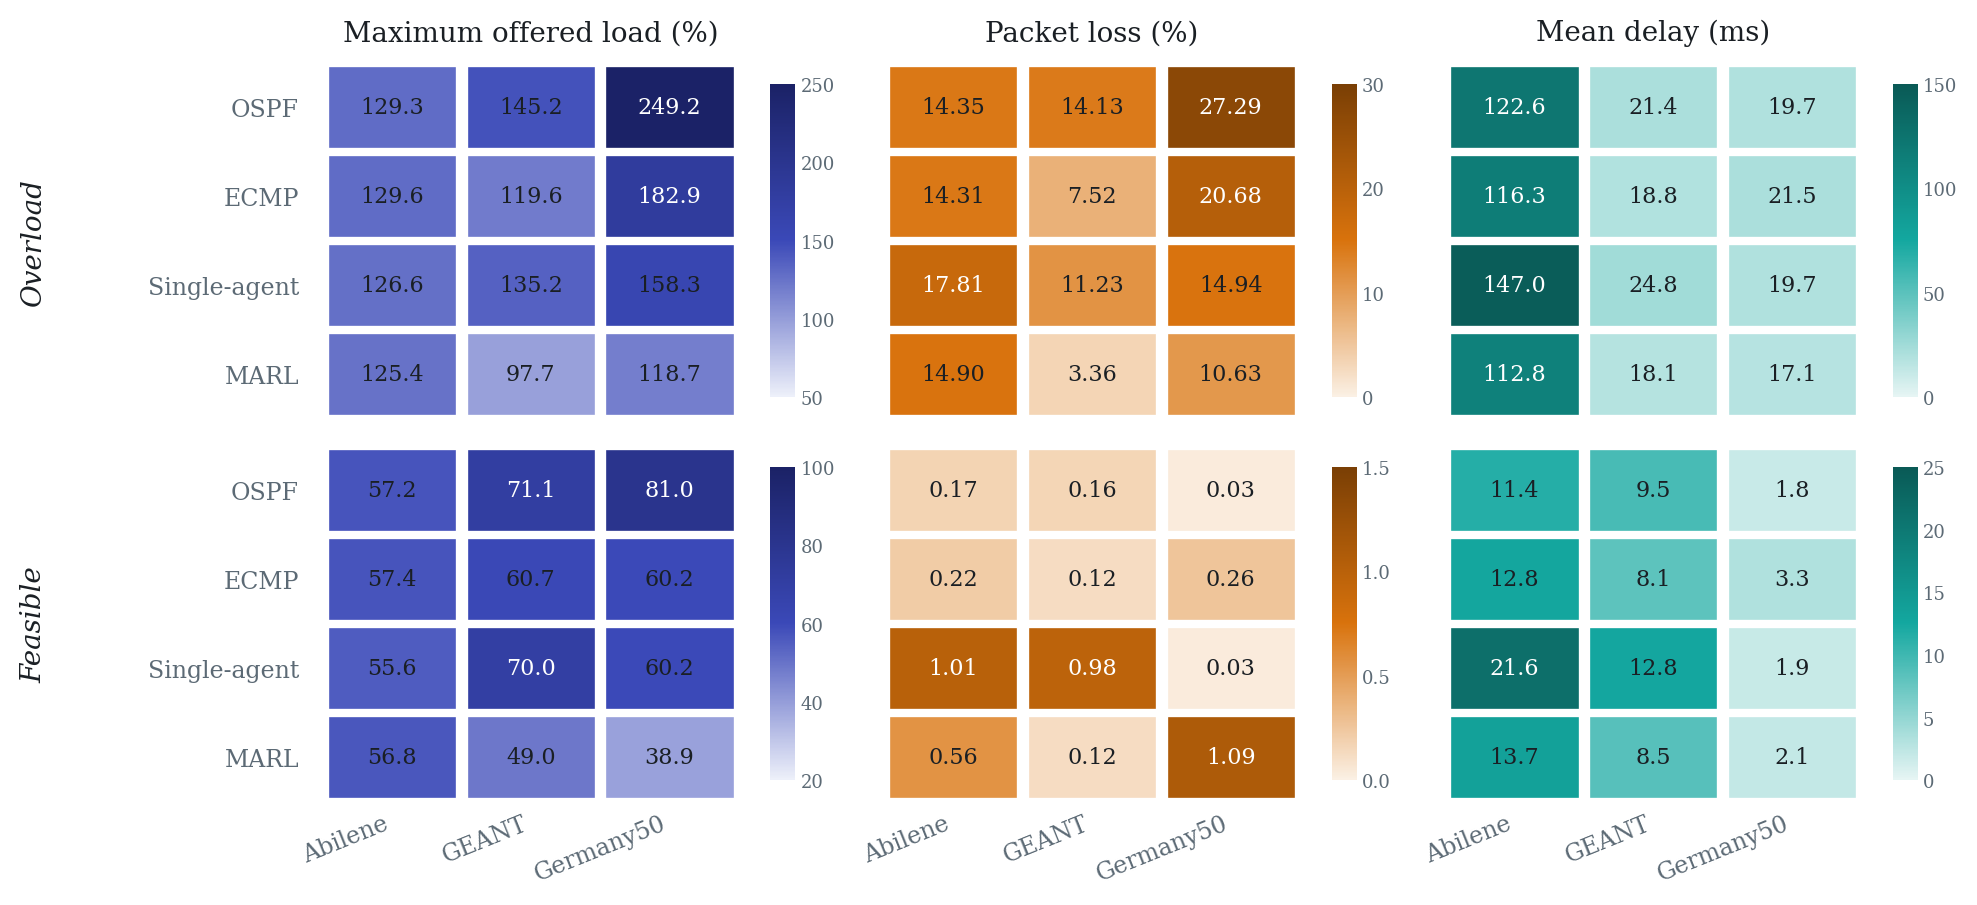
\includegraphics[width=\textwidth]{images/fig_heatmap_summary.png}
  \caption{Maximum offered load, packet loss and mean delay for the four methods
  on the three evaluation backbones, by congestion regime. Each metric is shaded
  within its own panel, so colour reads as distance from the best method on that
  network; absolute values are printed in every cell. Means over three model
  seeds.}
  \label{fig:heatmap}
\end{figure}

\subsection{Reward Trade-offs on Unseen Topologies}
\label{sec:res-reward}

The policy was trained on seventeen SNDLib topologies across three random seeds and then evaluated on three previously unseen topologies: Abilene, GÉANT, and Germany50 (training convergence is reported in Appendix~\ref{app:training}). The objective of this evaluation was to assess the trade-offs between performance gains and associated costs when applying the policy to new networks; Table~\ref{tab:reward-decomp} decomposes the resulting return into its congestion and delay terms. On Abilene, the policy detours on only $3.0\%$ of hops, incurs a cost of $4.8$, and reduces the bottleneck to $96\%$ of OSPF's bottleneck. On GÉANT, the policy detours on $3.8\%$ of hops, with a cost of $8.4$, reducing the bottleneck to $67\%$ of OSPF's. On Germany50, the largest improvement is observed, with the bottleneck reduced to $47\%$ of OSPF's, at the expense of detouring on $14.2\%$ of hops and a cost of $61.0$.

The trade is struck very differently across the three networks. On Abilene and GÉANT the return is dominated by the congestion term and the delay penalty is small, but on Germany50 the delay penalty is the larger of the two: the policy achieves its best bottleneck reduction there, to $47\%$ of OSPF's, yet pays enough detour hops that its overall return falls below the $-100$ that OSPF scores by construction. Lower bottleneck utilization is therefore not free.

These results indicate that the policy can be applied to other networks. Evaluation on previously unseen topologies demonstrates the trade-offs associated with the method employed in this study. Additional training with more steps, diverse topologies, and varied traffic patterns may further enhance model performance.

\subsection{Bottleneck Offered Load}
\label{sec:res-util}

Measured traffic data from SNDLib \citep{SNDlib10} provides actual traffic values across multiple timeframes. Traffic scaling is applied to generate demand for simulation. The resulting load is simulated on an analytical surrogate domain, since ns-3 link capacity is limited to 100\%. Therefore, simulation demand is evaluated under two distinct conditions: overload and feasible regimes. Results for both regimes are reported for all three networks.

Figure~\ref{fig:link-utilization} breaks the offered-load panel of Figure~\ref{fig:heatmap} out by topology, with the underlying values listed in Table~\ref{tab:offered-util}. The results show that MARL consistently outperforms other methods in both overload and feasible regimes. MARL achieves superior performance compared to OSPF, ECMP, and single-agent approaches on the GEANT and Germany50 networks, although it performs slightly worse than the single-agent method on Abilene. Additionally, MARL demonstrates a significant reduction in maximum offered load, achieving up to a 53\% decrease on GEANT and Germany50 in both regimes. In the overload regime, MARL reduces the offered load to 96.6\%, maintaining it below the 100\% threshold.

In the feasible regime, OSPF reaches a maximum offered load of 81\% on Germany50, while ECMP achieves 70.4\%. ECMP's more efficient algorithm results in approximately an 11\% reduction on both GEANT and Germany50 in the feasible regime. The single-agent approach shows significant improvement on Germany50 at 52\%, but underperforms on GEANT at 70\%. MARL outperforms all three baselines on GEANT and Germany50, achieving 48.2\% and 40.9\%, respectively.

The overload regime yields results similar to those observed in the feasible regime. Both the single-agent and MARL approaches improve routing decision performance in this regime. The single-agent method outperforms OSPF and ECMP on Abilene and Germany50, with improvements of 10\% and 29\%, respectively. MARL also demonstrates significant improvement by reducing the maximum offered load on GEANT and Germany50 to 96.6\% and 117\%, respectively.

These observations demonstrate that MARL improves routing by reducing the maximum offered load across both overload and feasible regimes. MARL also outperforms the single-agent approach on GEANT and Germany50. In two out of three networks, across both regimes, MARL distributes traffic more effectively than OSPF, ECMP, and single-agent methods. Therefore, the objective of using MARL to lower the bottleneck achieved.  



\begin{figure}[htbp]
  \centering
  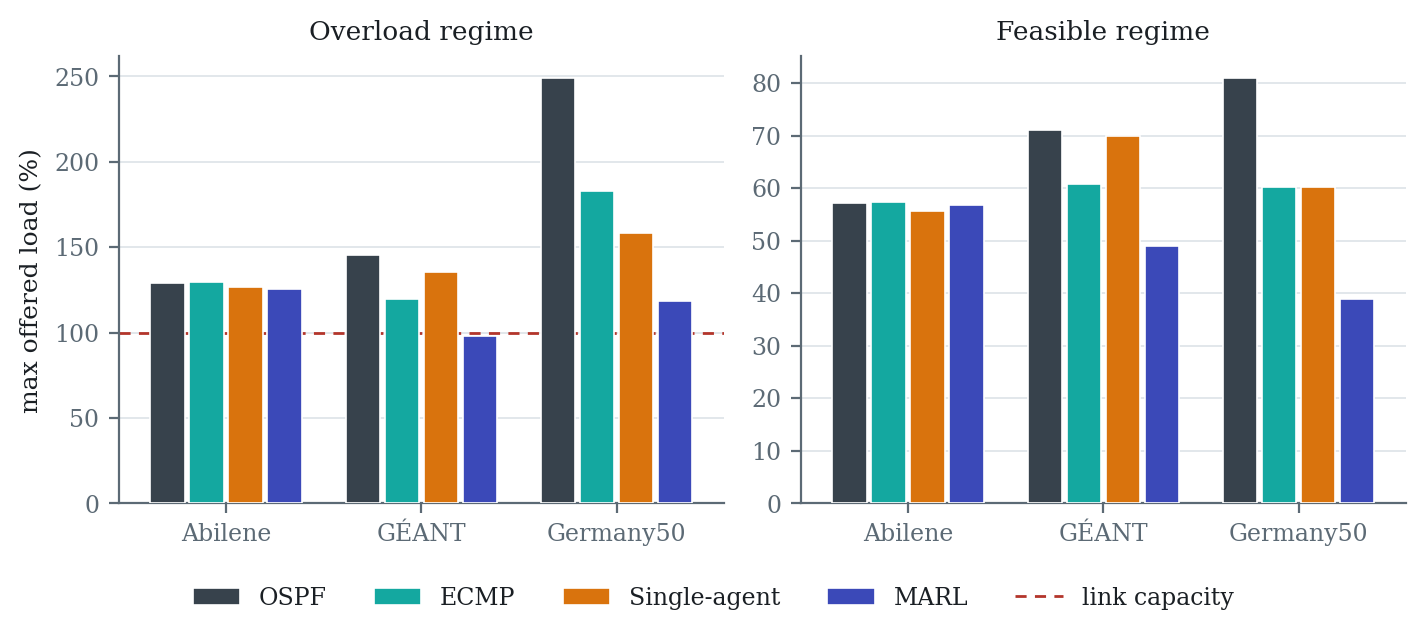
\includegraphics[width=0.8\textwidth]{images/fig_offered_util_regime.png}
  \caption{Maximum offered load on the bottleneck link, by regime and topology.}
  \label{fig:link-utilization}
\end{figure}

% \subsection{Greedy References}
% \label{sec:res-greedy}

% Neither learned policy should be credited with what a simple heuristic on the same
% action space already achieves. Table~\ref{tab:greedy} scores the two greedy
% best-responses of Section~\ref{sec:setup-hyper} on the identical matrices. Both
% require global link state after every decision and the path-level variant requires
% the demand matrix in advance, so neither is deployable; they are bounds, not
% competitors.

% \begin{table}[htbp]
%   \centering
%   \small
%   \caption{Greedy best-responses against OSPF and the reported learned arms, as
%   maximum offered load (\%). The path-level greedy shares the centralized action
%   space, the hop-level greedy the decentralized one.}
%   \label{tab:greedy}
%   \setlength{\tabcolsep}{4.5pt}
%   \begin{tabular}{lccccc}
%     \toprule
%     Cell & OSPF & Greedy (hop) & Greedy (path) & Single-agent & MARL $h{=}32$ \\
%     \midrule
%     Abilene overload   & 129.3 & 403.8 & \textbf{111.3} & 116.3 & 124.9 \\
%     GÉANT overload     & 145.2 & 148.8 & \textbf{87.9}  & 133.7 & 96.6  \\
%     Germany50 overload & 249.2 & 168.5 & \textbf{116.4} & 176.3 & 117.0 \\
%     \midrule
%     Abilene feasible   & 57.2  & 182.2 & \textbf{49.4}  & 54.2  & 56.1  \\
%     GÉANT feasible     & 71.1  & 72.4  & \textbf{45.7}  & 70.0  & 48.2  \\
%     Germany50 feasible & 81.0  & 56.8  & \textbf{37.7}  & 52.3  & 40.9  \\
%     \bottomrule
%   \end{tabular}
% \end{table}

% The two references separate sharply, and the separation is informative.

% \emph{Acting greedily hop by hop is far worse than not trying at all.} The
% hop-level best-response is beaten by OSPF on four of six cells and is
% catastrophic on Abilene, reaching $403.8\%$ where OSPF sits at $129.3\%$: choosing
% the locally least-congested next hop repeatedly walks a demand into a long path
% that loads links no single decision was accountable for. That the decentralized
% policy, acting in exactly this space, instead reaches $124.9\%$ and $96.6\%$ is
% the clearest evidence in this chapter that it has learned something beyond
% greed --- on GÉANT overload it improves on greedy by $52$ percentage points, and
% on Abilene by $279$.

% \emph{Acting greedily over whole paths is very strong.} The path-level
% best-response is the best arm in every cell, and by margins that are not small on
% GÉANT ($87.9$ against MARL's $96.6$) and Abilene ($111.3$ against the centralized
% policy's $116.3$). Only on Germany50 does a learned policy match it, MARL reaching
% $117.0$ against $116.4$. This bounds the contribution honestly: at $50$ nodes the
% learned policy is at the ceiling that its action space permits, while at $22$ and
% $12$ nodes a clairvoyant heuristic still does better. The gap is not evidence that
% the policies are under-trained --- they are at a matched budget and their seeds
% agree --- but that a policy acting on local observations, without the demand matrix
% and without recomputing global state per decision, pays something for that
% restriction. What it buys in exchange is the ability to run at all in a real
% network, where neither greedy reference could.

\subsection{Packet-Level Quality of Service}
\label{sec:res-qos}
Quality of Service results were obtained using the NS-3 simulator. FlowMonitor was employed to collect data from this packet-level simulator. To ensure consistency, measured traffic from SNDLib was used under maximum offered load conditions. The results are divided into overload and feasible regimes to highlight differences between these conditions. Packet loss is reported as a percentage, and delay is measured in milliseconds (ms). Table~\ref{tab:qos} lists the complete set of packet-level measurements, and Figures~\ref{fig:loss-qos} and~\ref{fig:delay-qos} break the corresponding panels of Figure~\ref{fig:heatmap} out by topology.

Overall, MARL is the strongest method in the overload regime, leading on four of the six loss and delay measurements. It achieves the lowest packet loss and delay at GEANT and demonstrates superior delay performance at Abilene and packet loss at Germany50. MARL reduces packet loss to 2.92\% at GEANT. However, as shown in Figure \ref{fig:loss-qos} and Figure \ref{fig:delay-qos}, loss and delay results are similar across methods in the feasible regime, with both MARL and ECMP achieving a packet loss of 0.12\% at GEANT.

MARL demonstrates strong performance in the overload regime by outperforming other methods in four out of six metrics. Specifically, it reduces delay to 108.8 ms at Abilene and 18.1 ms at GEANT under bottleneck traffic conditions. MARL also achieves the lowest packet loss at Germany50, with a value of 10.62\%. In contrast, the single-agent method achieves the lowest packet loss at Abilene (13.41\%), and ECMP achieves the lowest delay at Germany50 (17 ms).

In contrast, results in the feasible regime do not indicate significant differences in quality of service among the methods. Several metrics are identical across topologies and methods. For example, OSPF and ECMP both achieve a delay of 11.5 ms at Abilene, ECMP and MARL both record a packet loss of 0.12\% at GEANT, and OSPF and the single-agent method both achieve a packet loss of 0.03\% at Germany50. In this regime, packet loss varies only between 0.03 and 1.02\%, and delay ranges from 1.8 to 14.2 ms.

Quality of Service measurements demonstrate that MARL provides improved performance in the overload regime. The observed delay and packet loss are influenced by the routing protocol, particularly when hops increase or bottleneck traffic occurs. The study's objective is achieved, with the additional observation that in the feasible regime, baseline protocols such as OSPF and ECMP already provide sufficient performance.

\begin{figure}[htbp]
  \centering
  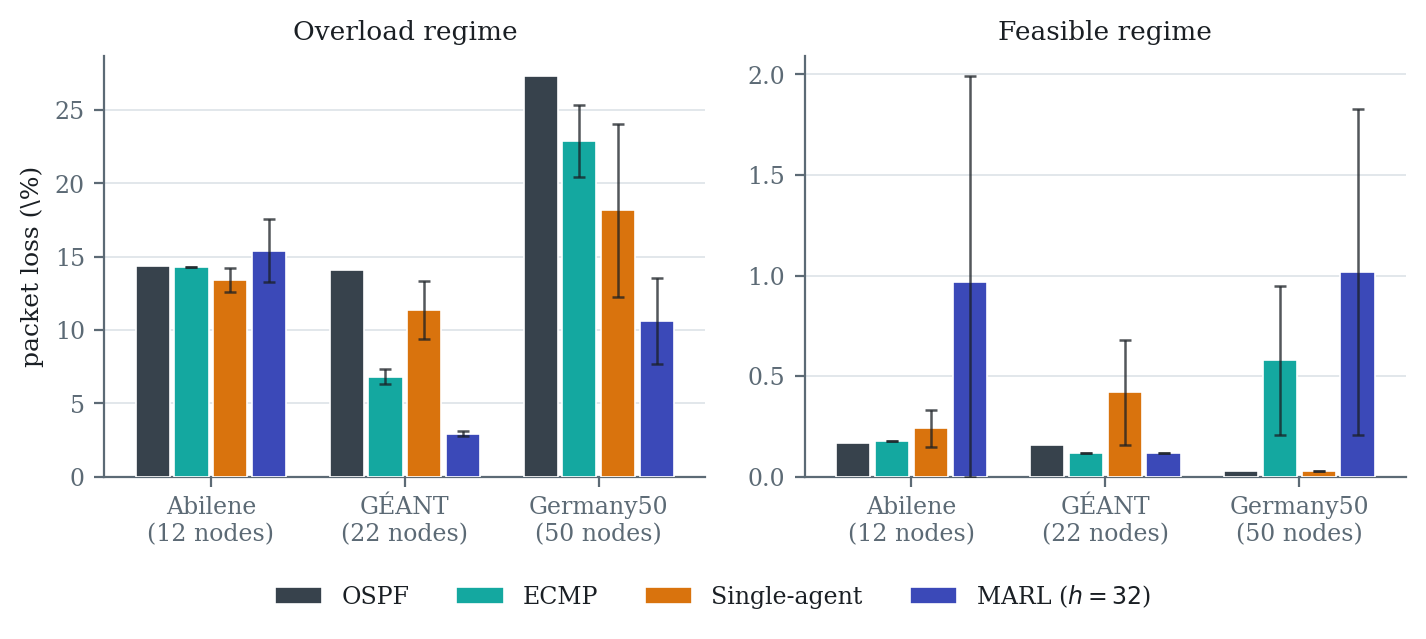
\includegraphics[width=0.8\textwidth]{images/fig_qos_loss_regime.png}
  \caption{Packet loss measured by ns-3 FlowMonitor, split by regime.}
  \label{fig:loss-qos}
\end{figure}

\begin{figure}[htbp]
  \centering
  
\includegraphics[width=0.8\textwidth]{images/fig_qos_delay_regime.png}
  \caption{Mean end-to-end delay measured by ns-3 FlowMonitor, split by regime.}
  \label{fig:delay-qos}
\end{figure}

% \subsection{Seed Stability and the Architectural Comparison}
% \label{sec:res-stability}

% Because all four learned arms now share identical PPO hyperparameters, the
% dispersion across seeds is a property of the architecture. The centralized policy
% is markedly the less stable of the two on the largest network: $\pm 51.4$
% percentage points of offered load on Germany50 against $\pm 3.5$ for MARL at
% $h{=}32$, and $\pm 5.90$ percentage points of packet loss against MARL's
% $\pm 2.91$. Inspection of the individual seeds shows the mechanism: one
% centralized seed collapses onto shortest-path selection, choosing the
% cost-shortest of the $k=3$ candidates for almost every demand, which reproduces
% OSPF and inflates the mean without inflating the training return. Across the
% evaluation networks the centralized policy routes $62$--$95\%$ of demands on
% exactly the OSPF path, against $47$--$80\%$ for MARL, so the collapse is a matter
% of degree rather than an all-or-nothing failure. The decentralized policy, whose
% per-node action space is re-entered at every hop and whose deviations are
% therefore incremental rather than committing a whole path, is the more stable at
% scale. On Abilene the ordering reverses and the centralized policy is the tighter
% of the two ($\pm 0.82$ against $\pm 2.13$ points of loss), which is consistent
% with it being the stronger arm there.

% This reverses the expectation that a $50$-node network would be hardest for a
% decentralized learner through multi-agent credit assignment, with each agent's
% return depending on forty-nine others whose policies change concurrently. That
% effect is real but is evidently not the binding constraint at this scale: MARL is
% the stronger architecture on Germany50 under overload by $7.6$ to $9.3$ points of
% loss. What survives of the scale argument is confined to the feasible regime,
% where hop-by-hop construction produces routes that free headroom at a small but
% consistent cost in loss, and where the centralized formulation's global view of a
% whole path is the better tool.

% The reported width, $h{=}32$, was selected on the \emph{training} topologies
% (Section~\ref{sec:setup-hyper}) and not on any evidence in this chapter. A wider
% $h{=}64$ variant was trained and evaluated identically as the alternative
% candidate; it was not selected and is not reported. Its behaviour is consistent
% with the choice: it carries roughly three times the seed dispersion of $h{=}32$
% ($\pm 3.0$ against $\pm 1.6$ on GÉANT overload, $\pm 9.7$ against $\pm 3.5$ on
% Germany50) and is the only configuration tested that is worse than OSPF on any
% cell.

% Against the centralized controller the two architectures split the six cells
% evenly. MARL takes both GÉANT cells and Germany50 overload --- the three in which
% the network is large or the demand heavy --- by $8.5$, $27.7$ and $7.6$ points
% respectively. The centralized controller takes both Abilene cells and Germany50
% feasible, the three in which OSPF is already close to optimal and the useful
% deviations are few. The pattern is consistent with the mechanism argued above:
% incremental per-hop diversification pays when there is slack to redistribute, and
% whole-path selection pays when only a handful of targeted changes are worth
% making.

% That split is worth reading alongside the parameter counts of
% Table~\ref{tab:hyper}. The reported decentralized policy carries $17{,}570$
% trainable parameters against the centralized controller's $268{,}420$, a factor
% of fifteen. Whatever advantage the decentralized formulation confers where it
% wins, it is not bought with capacity.

% \subsection{Where the Decentralized Method Fails: Abilene}
% \label{sec:res-abilene}

% Abilene is where the decentralized formulation loses, and it is the one network on
% which the ranking of the two learned architectures inverts. MARL at $h{=}32$
% records $0.97\%$ loss and $14.2$\,ms delay in the feasible regime against OSPF's
% $0.17\%$ and $11.5$\,ms, and $15.41\%$ loss in overload against OSPF's $14.35\%$.
% The centralized
% controller, by contrast, matches OSPF's service in the feasible regime ($0.24\%$
% loss, $13.8$\,ms) while holding the bottleneck $8.5$ points lower at $88.1\%$,
% and takes the lowest loss in the cell under overload, $13.41\%$ against OSPF's
% $14.35\%$ and ECMP's $14.30\%$.

% So the negative result is specific rather than general: \emph{learned routing}
% improves on OSPF at twelve nodes, but the hop-by-hop decentralized formulation
% does not. Two properties of the network explain the asymmetry. First, Abilene is
% the only evaluation instance with heterogeneous link capacities, fourteen links at
% $9.92$\,Gbps and one at $2.48$\,Gbps; correctly costed, OSPF prices that link at
% four and routes around it almost entirely, so the baseline is already close to
% optimal and the margin available to any optimiser is thin. Second, with only
% twelve nodes and $132$ demand pairs there is little scope for the incremental,
% per-hop diversification that is MARL's advantage on larger networks, while its
% per-hop detour penalty still accumulates. The centralized controller, choosing
% whole cost-shortest paths, expresses exactly the small number of targeted
% deviations that this network rewards.

% This bounds the contribution in a useful way. The decentralized formulation's
% value is concentrated in networks large enough, or loaded heavily enough, that
% shortest-path routing leaves genuine slack on the table: it wins by $11.2$ points
% of loss at twenty-two nodes and by $8.6$ at fifty, and loses by roughly one point
% at twelve. The crossover lies below the scale of any of the three backbones
% studied, which is a more informative statement than a uniform win would have been.



% \subsection{Limitations}
% \label{sec:res-limitations}

% Six limitations qualify these results.

% The policies are trained against an analytical link-utilisation surrogate rather
% than ns-3, since packet-level simulation is too slow inside a training loop. The
% agreement between objective and measurement in the overload regime shows the
% surrogate is adequate there, but it does not guarantee untested regimes, and the
% Germany50 feasible cell is precisely a case where the surrogate's ranking and the
% packet-level ranking disagree.

% The Germany50 OSPF baseline is sensitive to equal-cost tie-breaking. Germany50's
% links are of uniform capacity, so weighting the metric does not change any path
% cost; it changes only which of several equal-cost paths the shortest-path
% computation returns. That choice alone moves OSPF's measured overload loss by
% several percentage points, and it moves in the direction that flatters the
% learned policies. The Germany50 margins should be read with this in mind.

% The reward comparison of Section~\ref{sec:res-reward} was run for the
% centralized architecture only. Whether the decentralized policy would likewise
% improve under the centralized reward form was not tested, so the claim is that
% the reported baseline is the stronger of two configurations, not that it is
% optimal.

% Three seeds is few, particularly given the dispersion documented in
% Section~\ref{sec:res-stability}. The Germany50 feasible utilisation figures carry
% seed standard deviations between $\pm 13$ and $\pm 20$ percentage points, and
% differences between arms within that cell are not resolved by this evidence.

% Abilene's two tables describe the same policies at different operating points, for
% the reason given in Section~\ref{sec:setup-scaling}, and should not be read
% across. Similarly, the absolute Germany50 figures correspond to the top $200$ of
% $2450$ demand pairs; all methods see the identical flow set, so the comparison is
% unbiased, but the magnitudes are those of that subset.

% Finally, topologies are static and each simulation holds a single traffic matrix.
% Link and node failures, convergence during a topology change, and adaptation to
% traffic shifting \emph{within} an episode are not evaluated. The study
% demonstrates generalisation across networks and across matrices, not adaptation
% within one, and this remains the largest gap between the present work and a
% deployable system.
